% Options for packages loaded elsewhere
\PassOptionsToPackage{unicode}{hyperref}
\PassOptionsToPackage{hyphens}{url}
%
\documentclass[
]{article}
\usepackage{amsmath,amssymb}
\usepackage{stata}
\usepackage{lmodern}
\usepackage{iftex}
\ifPDFTeX
  \usepackage[T1]{fontenc}
  \usepackage[utf8]{inputenc}
  \usepackage{textcomp} % provide euro and other symbols
\else % if luatex or xetex
  \usepackage{unicode-math}
  \defaultfontfeatures{Scale=MatchLowercase}
  \defaultfontfeatures[\rmfamily]{Ligatures=TeX,Scale=1}
\fi
% Use upquote if available, for straight quotes in verbatim environments
\IfFileExists{upquote.sty}{\usepackage{upquote}}{}
\IfFileExists{microtype.sty}{% use microtype if available
  \usepackage[]{microtype}
  \UseMicrotypeSet[protrusion]{basicmath} % disable protrusion for tt fonts
}{}
\makeatletter
\@ifundefined{KOMAClassName}{% if non-KOMA class
  \IfFileExists{parskip.sty}{%
    \usepackage{parskip}
  }{% else
    \setlength{\parindent}{0pt}
    \setlength{\parskip}{6pt plus 2pt minus 1pt}}
}{% if KOMA class
  \KOMAoptions{parskip=half}}
\makeatother
\usepackage{xcolor}
\IfFileExists{xurl.sty}{\usepackage{xurl}}{} % add URL line breaks if available
\IfFileExists{bookmark.sty}{\usepackage{bookmark}}{\usepackage{hyperref}}
\hypersetup{
  pdftitle={Why Stata Is Better (At Graphing) Than R},
  pdfauthor={Andy Grogan-Kaylor},
  hidelinks,
  pdfcreator={LaTeX via pandoc}}
\urlstyle{same} % disable monospaced font for URLs
\usepackage[margin=1 in]{geometry}
\usepackage{graphicx}
\makeatletter
\def\maxwidth{\ifdim\Gin@nat@width>\linewidth\linewidth\else\Gin@nat@width\fi}
\def\maxheight{\ifdim\Gin@nat@height>\textheight\textheight\else\Gin@nat@height\fi}
\makeatother
% Scale images if necessary, so that they will not overflow the page
% margins by default, and it is still possible to overwrite the defaults
% using explicit options in \includegraphics[width, height, ...]{}
\setkeys{Gin}{width=\maxwidth,height=\maxheight,keepaspectratio}
% Set default figure placement to htbp
\makeatletter
\def\fps@figure{htbp}
\makeatother
\setlength{\emergencystretch}{3em} % prevent overfull lines
\providecommand{\tightlist}{%
  \setlength{\itemsep}{0pt}\setlength{\parskip}{0pt}}
\setcounter{secnumdepth}{-\maxdimen} % remove section numbering
\ifLuaTeX
  \usepackage{selnolig}  % disable illegal ligatures
\fi

\title{Why Stata Is Better (At Graphing) Than R}
\author{Andy Grogan-Kaylor}
\date{7 Apr 2022 15:43:09}

\begin{document}
\maketitle

Both R and Stata are programs with strong data visualization and
analysis capabilities. However, Stata's capabilities as a data
visualization program are sometimes under-rated. The intent of the post
is to show that Stata can often perform the same graphing task as R,
with much simpler, and much more intuitive, command syntax.

This post uses simulated social service agency data clients. In each
program, I am going to graph mental health of clients (at Time 2) by
program.

\hypertarget{stata}{%
\section{Stata}\label{stata}}

\begin{stlog}
. import delimited "clients.csv", encoding(ISO-8859-2) clear // import data
(8 vars, 491 obs)
{\smallskip}
.     
. graph bar mental_health_t2, over(program) scheme(michigan) asyvars // bar graph of m
> ental health over program
\end{stlog}



\begin{figure}
\centering
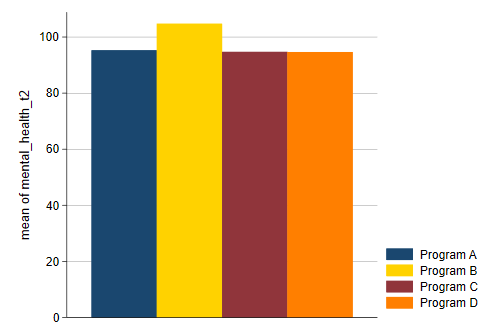
\includegraphics[width=0.75\linewidth]{mybarStata.png}
\caption{Bar Graph in Stata}
\end{figure}

\hypertarget{r}{%
\section{R}\label{r}}

\begin{stlog}
> library(readr) \# library to import data
>     
> clients <- read_csv("clients.csv") \# import data
>     
> library(ggplot2)
>     
> library(michigancolors)
> 
> ggplot(clients, \# the data that I am using
+   aes(x = program, \# 'aesthetic' includes x
+       y = mental_health_T2, \# and y
+       fill = program)) + 
+   stat_summary(fun = mean, \# summarizing y 
+                geom = "bar") + \# with bars
+   scale_fill_manual(values = michigancolors()) +
+   theme(axis.text.x = element_text(size = rel(.3)))
\end{stlog}



\begin{figure}
\centering
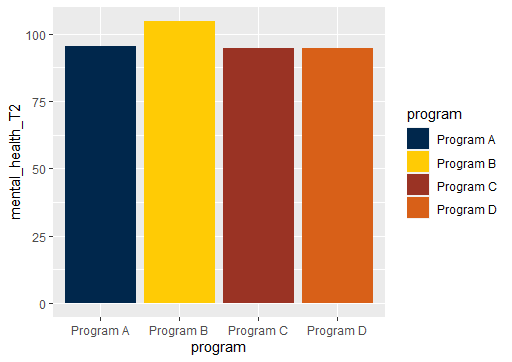
\includegraphics[width=0.75\linewidth]{mybarR.png}
\caption{Bar Graph in R}
\end{figure}

\end{document}
